\chapter{Weryfikacja i walidacja}
\label{ch:06}

Z uwagi na implementację programu na karcie graficznej jako jednostkę cieniującą fragmentów, weryfikacja poprawności jego działania jest znacznie utrudniona. Programując w języku GLSL, brak jest możliwości zastosowania testów jednostkowych, co spowodowało, że testowanie sprowadzało się do działań metodą prób i błędów. Przeprowadzono porównania różnych technik i wzorów, by uzyskać pożądany efekt. Ewentualne niepoprawne obliczenia są często niewidoczne, mimo wydawałoby się poprawnego działania. Jednym z takich problemów było obliczanie wektorów normalnych powierzchni, co spowodowane było niepoprawnym zastosowaniem wzoru. Błąd ten ujawnił się dopiero po implementacji cieni, gdy oświetlone powierzchnie były przyciemnione, sprawiały wrażenie, że były odwrócone od źródła światła. Defekt ten przedstawia rysunek \ref{fig:normals}.

\begin{figure}[H]
\centering
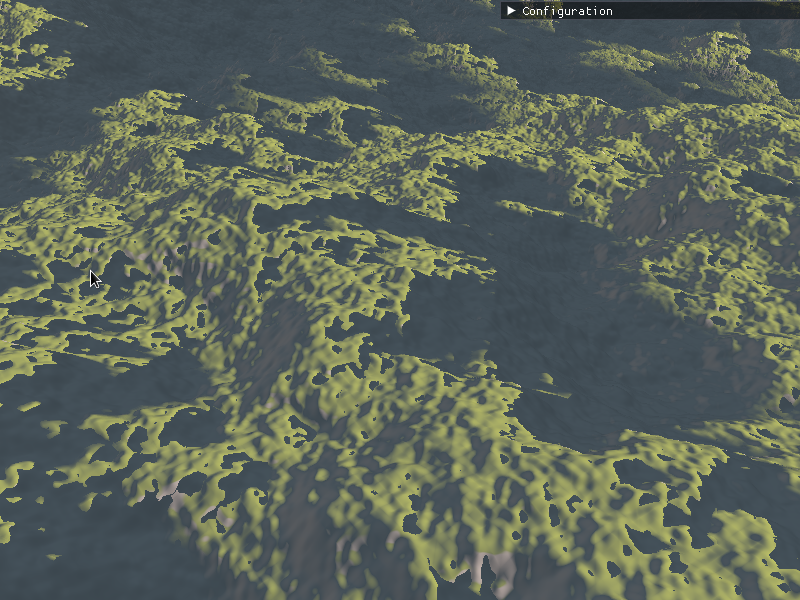
\includegraphics[width=0.76\textwidth]{./graf/norm.png}
\caption{Niepoprawne obliczanie wektorów normalnych.}
\label{fig:normals}
\end{figure}

Kolejnym problemem związanym z implementacją programu na karcie graficznej jest utrudniona weryfikacja wydajności zaimplementowanych funkcji ze względu na brak narzędzi przeznaczonych do tego celu. Przykładem takiej sytuacji było renderowanie drzew, które znacząco spowalniało działanie programu.
Aby wyjaśnić przyczynę tego zjawiska, zaimplementowano wizualizację przybliżonego czasu działania algorytmu raymarching poprzez przedstawienie ilości iteracji algorytmu jako barwę. Przyjęto, że~kolor niebieski oznacza minimalną ilość kroków, a kolor czerwony maksymalną ilość kroków, wyznaczoną przez użytkownika. Wizualizacja tego typu nie jest jednak idealnym odwzorowaniem czasu działania algorytmu, gdyż poszczególne elementy sceny różnią się ilością czasu potrzebnego do wykonania ich obliczeń. Mimo to, taka wizualizacja pozwala~na zdiagnozowanie ewentualnych problemów związanych z~wydajnością algorytmu. Porównanie uzyskanych wyników dla terenu bez drzew oraz z~drzewami, znajduje odzwierciedlenie na rysunku \ref{fig:iters}.

\begin{figure}[H]
\centering
\subfloat[Teren bez drzew]{
  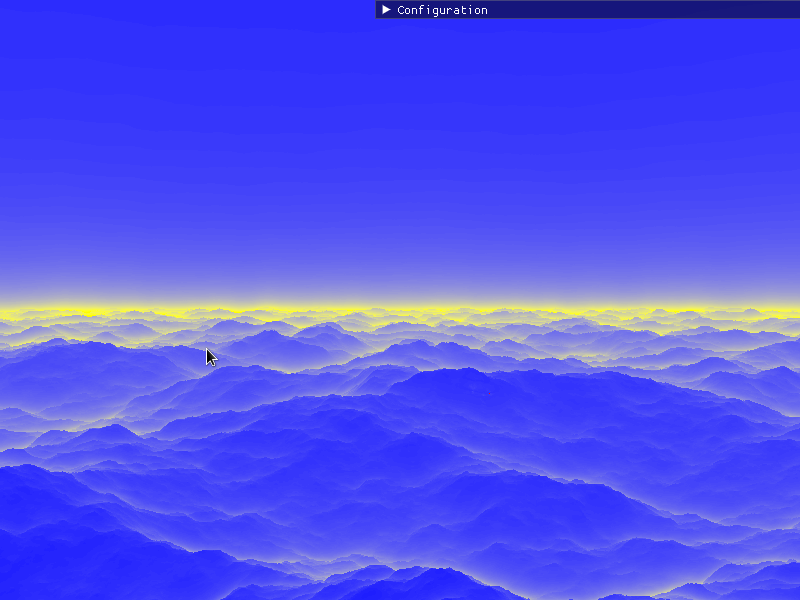
\includegraphics[width=0.5\textwidth]{./graf/iterations-notrees.png}
%%   \label{fig:lerp}
}
\subfloat[Teren oraz drzewa]{
  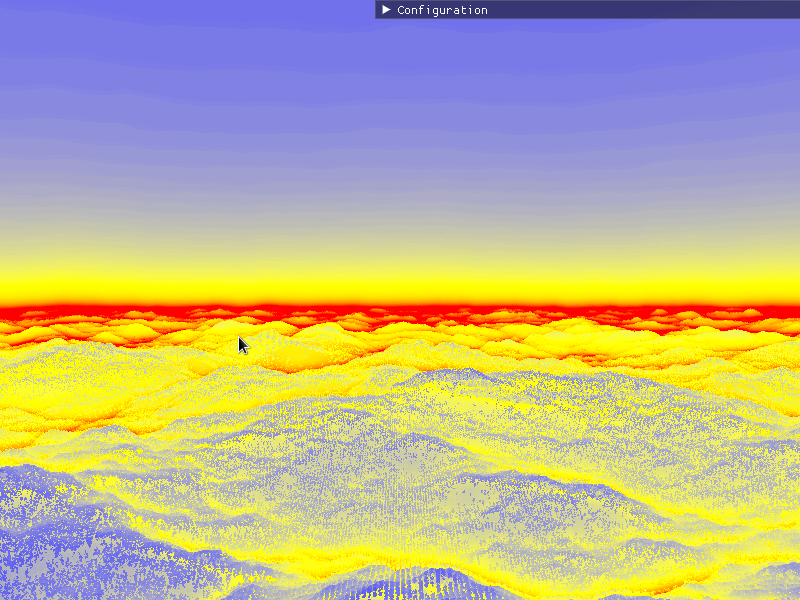
\includegraphics[width=0.5\textwidth]{./graf/iterations-trees-unopt.png}
  \label{fig:iters-tree}
}
%% 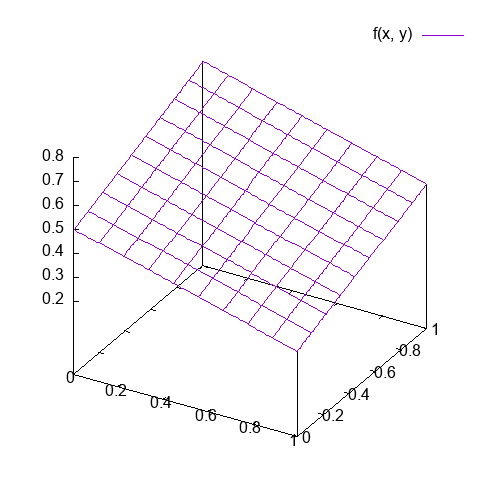
\includegraphics[width=0.65\textwidth]{./graf/plot/bilinear.png}
\caption{Porównanie ilości kroków renderowania. Kolor czerwony przedstawia 255 iteracji algorytmu.}
\label{fig:iters}
\end{figure}

Rysunek \ref{fig:iters-tree} udawadnia, że przy obecnej implementacji większość iteracji wykonywana jest w dużej odległości od kamery, gdzie drzewa są praktycznie niewidoczne. W celu uniknięcia tego efektu ograniczono maksymalną odległość renderowania drzew oraz przyznano użytkownikowi możliwość kontroli nad tym parametrem. Wynik zastosowania powyższej optymalizacji został przedstawiony na~rysunku \ref{fig:iters-opt}.

\begin{figure}[H]
\centering
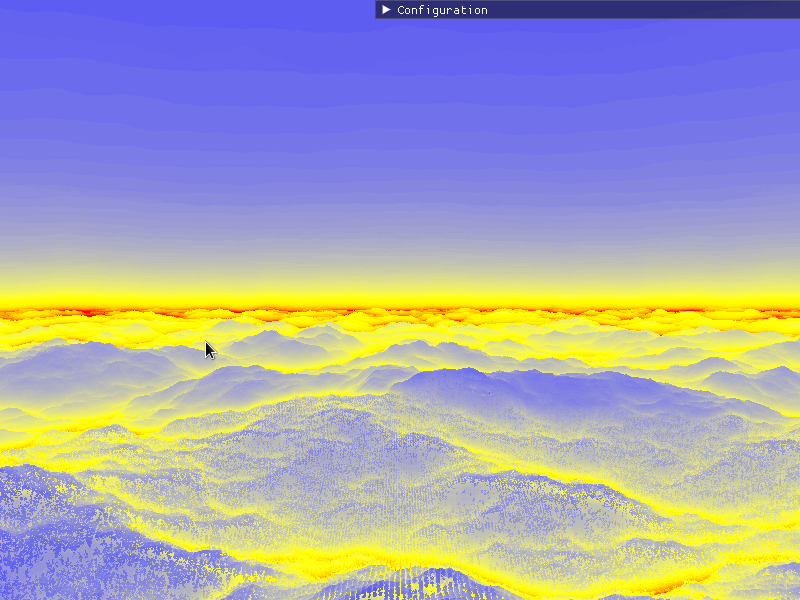
\includegraphics[width=1\textwidth]{./graf/iterations-trees-opt.png}
\caption{Wizualizacja iteracji algorytmu po optymalizacji. Kolor czerwony przedstawia 255 iteracji.}
\label{fig:iters-opt}
\end{figure}



%% \begin{itemize}
%% \item sposób testowania w ramach pracy (np. odniesienie do modelu V)
%% \item organizacja eksperymentów
%% \item przypadki testowe zakres testowania (pełny/niepełny)
%% \item wykryte i usunięte błędy
%% \item opcjonalnie wyniki badań eksperymentalnych
%% \end{itemize}

%% \begin{table}
%% \centering
%% \caption{Nagłówek tabeli jest nad tabelą.}
%% \label{id:tab:wyniki}
%% \begin{tabular}{rrrrrrrr}
%% \toprule
%% 	         &                                     \multicolumn{7}{c}{metoda}                                      \\
%% 	         \cmidrule{2-8}
%% 	         &         &         &        \multicolumn{3}{c}{alg. 3}        & \multicolumn{2}{c}{alg. 4, $\gamma = 2$} \\
%% 	         \cmidrule(r){4-6}\cmidrule(r){7-8}
%% 	$\zeta$ &     alg. 1 &   alg. 2 & $\alpha= 1.5$ & $\alpha= 2$ & $\alpha= 3$ &   $\beta = 0.1$  &   $\beta = -0.1$ \\
%% \midrule
%% 	       0 &  8.3250 & 1.45305 &       7.5791 &    14.8517 &    20.0028 & 1.16396 &                       1.1365 \\
%% 	       5 &  0.6111 & 2.27126 &       6.9952 &    13.8560 &    18.6064 & 1.18659 &                       1.1630 \\
%% 	      10 & 11.6126 & 2.69218 &       6.2520 &    12.5202 &    16.8278 & 1.23180 &                       1.2045 \\
%% 	      15 &  0.5665 & 2.95046 &       5.7753 &    11.4588 &    15.4837 & 1.25131 &                       1.2614 \\
%% 	      20 & 15.8728 & 3.07225 &       5.3071 &    10.3935 &    13.8738 & 1.25307 &                       1.2217 \\
%% 	      25 &  0.9791 & 3.19034 &       5.4575 &     9.9533 &    13.0721 & 1.27104 &                       1.2640 \\
%% 	      30 &  2.0228 & 3.27474 &       5.7461 &     9.7164 &    12.2637 & 1.33404 &                       1.3209 \\
%% 	      35 & 13.4210 & 3.36086 &       6.6735 &    10.0442 &    12.0270 & 1.35385 &                       1.3059 \\
%% 	      40 & 13.2226 & 3.36420 &       7.7248 &    10.4495 &    12.0379 & 1.34919 &                       1.2768 \\
%% 	      45 & 12.8445 & 3.47436 &       8.5539 &    10.8552 &    12.2773 & 1.42303 &                       1.4362 \\
%% 	      50 & 12.9245 & 3.58228 &       9.2702 &    11.2183 &    12.3990 & 1.40922 &                       1.3724 \\
%% \bottomrule
%% \end{tabular}
%% \end{table}
